\documentclass[spanish]{beamer}
\usepackage[utf8]{inputenc}
\usepackage{float}
\usepackage{beamerthemesplit}
\usepackage{latexsym}
\usepackage[T1]{fontenc}
\usepackage{amsmath}
\usepackage{hyperref}
\usepackage{graphicx}
\usepackage{babel,blindtext}
\usepackage{amsfonts}
\usepackage[round]{natbib}
\bibliographystyle{chicago}
\usepackage{subcaption} 


\decimalpoint

%\documentclass{beamer}
\usetheme[pageofpages=of,% String used between the current page and the
                         % total page count.
          bullet=circle,% Use circles instead of squares for bullets.
          titleline=true,% Show a line below the frame title.
          alternativetitlepage=true,% Use the fancy title page.
          titlepagelogo=logo,% Logo for the first page.
          watermark=logo2,% Watermark used in every page.
          watermarkheight=60px,% Height of the watermark.
          watermarkheightmult=3,% The watermark image is 4 times bigger
                                % than watermarkheight.
          ]{Torino}

%
%\usetheme{Antibes}%este es el templete que se usa a lo largo de la presentacion
%%themes
%%   default
%%   Boadilla
%%   Madrid
%%   Pittsburgh
%%   Copenhagen
%%   Warsaw
%%   Singapore
%%   Malmoe
%\newcommand\Fontvi{\fontsize{6}{7.2}\selectfont}
\mode<presentation>%tipo de 
\begin{document}

%%%%%%%%%%%%%%%%%%%%%%%%%%%%%%%%%%%%%%%%%%%%%%%%%%%%%%%%%%%%%%%%%%%%%%%%%%%%%%%%%%%%%%%%%%%%%%%%%%%%%%%%%%%%%
\title{Descripción de datos con medidas numéricas}
\subtitle{Estadística}
\author{Gamaliel Moreno Chávez}
\institute{Centro de Crecimiento Humanista}
\date{Enero\\ 2021}%para que ponga la fecha de hoy 

\frame{\titlepage}
%%%%%%%%%%%%%%%%%%%%%%%%%%%%%%%%%%%%%%%%%%%%%%%%%%%%%%%%%%%%%%%%%%%%%%%%%%%%%%%%%%%%%%%%%%%%%%%%%%%%%%%%%%%%%
%%%%%%%%%%%%%%%%%%%%%%%%%%%%%%%%%%%%%%%%%%%%%%%%%%%%%%%%%%%%%%%%%%%%%%%%%%%%%%%%%%%%%%%%%%%%%%%%%%%%%%%%%%%%%%%%%%%%%%%%%%%%%%%%%%%%%%%%%%%%%%%%%%%%%%%%%%%%%%%%%%%%%%%%%%%%%%%%%%%%%%%%%%%%%%%%%%%%%%%%%%%%%%%%%%%%%%%%%%
%%%%%%%%%%%%%%%%%%%%%%%%%%%%%%%%%%%%%%%%%%%%%%%%%%%%%%%%%%%%%%%%%%%%%%%%%%%%%%%%%%%%%%%%%%%%%%%%%%%%%%%%%%%%%%%%%%%%%%%%%%%%%%%%%%%%%%%%%%%%%%%%%%%%%%%%%%%%%%%%%%%%%%%%%%%%%%%%%%%%%%%%%%%%%%%%%%%%%%%%%%%%%%%%%%%%%%%%%%

\begin{frame}
\frametitle{Generalidades}
Las gráficas pueden ayudar a describir la forma básica de una distribución de datos pero hay limitaciones
\begin{itemize}
\item No siempre es posible presentar gráficas.
\item Son poco precisas.
\item No son comparables
\end{itemize}
Una forma de superar estos problemas es usar medidas numéricas, que se pueden calcular para una muestra o una población de mediciones.
\end{frame}

%%%%%%%%%%%%%%%%%%%%%%%%%%%%%%%%%%%%%%%%%%%%%%%%%%%%%%%%%%%%%%%%%%%%%%%%%%%%%%%%%%%%%%%%%%%%%%%%%%%%%%%%%%%%%
\begin{frame}
\frametitle{Generalidades} 
\begin{block}{Definición}
Las mediciones descriptivas numéricas asociadas con una población de
mediciones se llaman parámetros; las calculadas a partir de mediciones muestrales reciben el nombre de estadísticas.
\end{block}
\end{frame}
%%%%%%%%%%%%%%%%%%%%%%%%%%%%%%%%%%%%%%%%%%%%%%%%%%%%%%%%%%%%%%%%%%%%%%%%%%%%%%%%%%%%%%%%%%%%%%%%%%%%%%%%%%%%%
\begin{frame}
\frametitle{Medidas de centro} 
Una de las primeras mediciones numéricas importantes es
una medida de centro, es decir, una medida a lo largo del eje horizontal que localiza el centro de la distribución.

\begin{center}
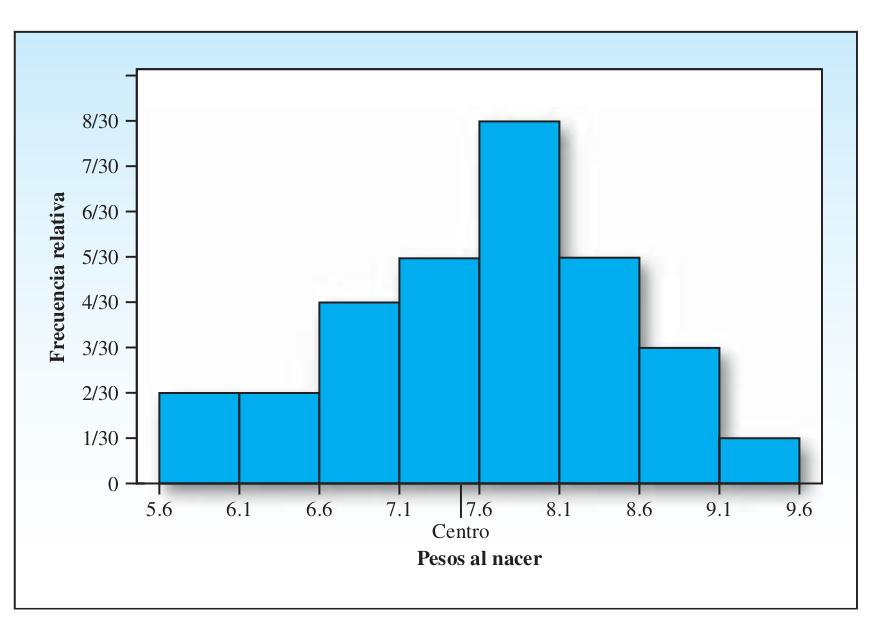
\includegraphics[scale=0.28]{im1}
\end{center}
\end{frame}
%%%%%%%%%%%%%%%%%%%%%%%%%%%%%%%%%%%%%%%%%%%%%%%%%%%%%%%%%%%%%%%%%%%%%%%%%%%%%%%%%%%%%%%%%%%%%%%%%%%%%%%%%%%%%
\begin{frame}
\frametitle{Media} 
El \textbf{promedio aritmético} de un conjunto de mediciones es una medida de centro muy común y útil. Se conoce como \textbf{media aritmética} o simplemente \textbf{media}. Para distinguirla usamos el símbolo $\bar{x}$ (x barra).



\begin{block}{Definición}
La media aritmética o promedio de un conjunto de n mediciones es
igual a la suma de las mediciones dividida entre n
\end{block}

\end{frame}
%%%%%%%%%%%%%%%%%%%%%%%%%%%%%%%%%%%%%%%%%%%%%%%%%%%%%%%%%%%%%%%%%%%%%%%%%%%%%%%%%%%%%%%%%%%%%%%%%%%%%%%%%%%%%
\begin{frame}
\frametitle{Media} 
\begin{center}
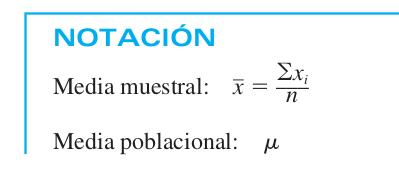
\includegraphics[scale=0.5]{im2}
\end{center}

\begin{equation*}
\sum_{i=1}^{n}{x_{i}} \text{  que significa } x_{1}+x_{2}+x_{3}+\cdots + x_{n}
\end{equation*}

$\sum {x_{i}}$ que significa “la suma de todas las mediciones de x”
\end{frame}

%%%%%%%%%%%%%%%%%%%%%%%%%%%%%%%%%%%%%%%%%%%%%%%%%%%%%%%%%%%%%%%%%%%%%%%%%%%%%%%%%%%%%%%%%%%%%%%%%%%%%%%%%%%%%
\begin{frame}
\frametitle{Media} 
Ejemplo
\begin{center}
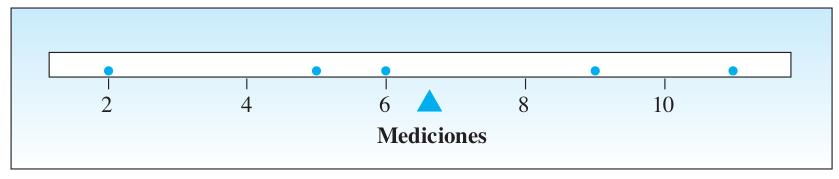
\includegraphics[scale=0.35]{im3}
\end{center}

\begin{equation*}
\bar{x}= \frac{\sum x_{i}}{n}= \frac{2+9+11+5+6}{5}=6.6
\end{equation*}

\end{frame}
%%%%%%%%%%%%%%%%%%%%%%%%%%%%%%%%%%%%%%%%%%%%%%%%%%%%%%%%%%%%%%%%%%%%%%%%%%%%%%%%%%%%%%%%%%%%%%%%%%%%%%%%%%%%%
\begin{frame}
\frametitle{Media} 
Ejercicio. Calcule la media para los siguientes datos

\begin{center}
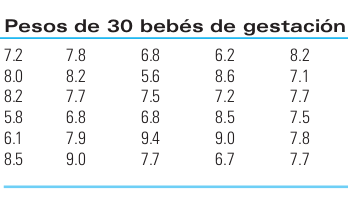
\includegraphics[scale=0.5]{im4}
\end{center}
\end{frame}
%%%%%%%%%%%%%%%%%%%%%%%%%%%%%%%%%%%%%%%%%%%%%%%%%%%%%%%%%%%%%%%%%%%%%%%%%%%%%%%%%%%%%%%%%%%%%%%%%%%%%%%%%%%%%
\begin{frame}
\frametitle{Mediana}

Una segunda medida de tendencia central es la mediana, que es el valor de la posición media en el conjunto de mediciones ordenada de menor a mayor.

\begin{block}{Definición}
La mediana m de un conjunto de n mediciones es el valor de x que cae
en la posición media cuando las mediciones son ordenadas de menor a mayor.
\end{block}

\end{frame}
%%%%%%%%%%%%%%%%%%%%%%%%%%%%%%%%%%%%%%%%%%%%%%%%%%%%%%%%%%%%%%%%%%%%%%%%%%%%%%%%%%%%%%%%%%%%%%%%%%%%%%%%%%%%%
\begin{frame}
\frametitle{Mediana}
Ejemplo 

\begin{center}
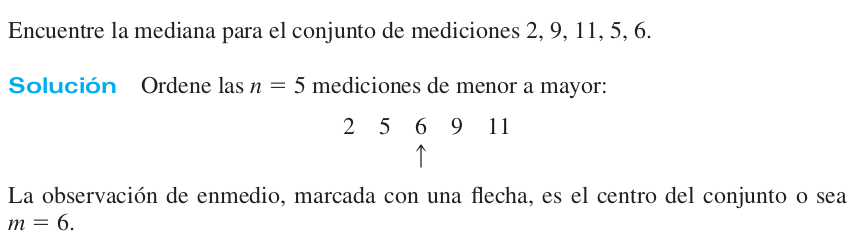
\includegraphics[width=\textwidth]{im5}
\end{center}


\end{frame}
%%%%%%%%%%%%%%%%%%%%%%%%%%%%%%%%%%%%%%%%%%%%%%%%%%%%%%%%%%%%%%%%%%%%%%%%%%%%%%%%%%%%%%%%%%%%%%%%%%%%%%%%%%%%%
\begin{frame}
\frametitle{Mediana}
Ejemplo 

\begin{center}
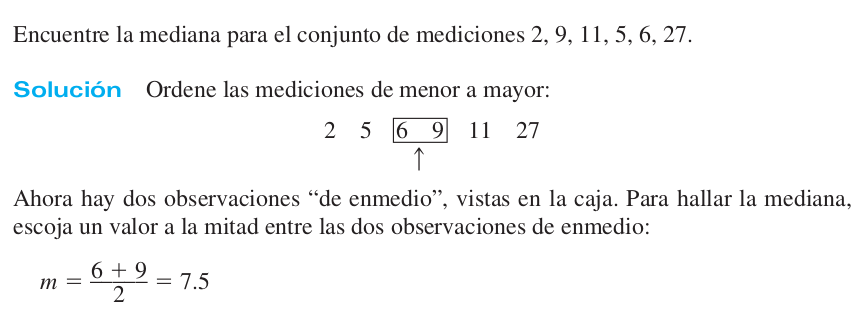
\includegraphics[width=\textwidth]{im6}
\end{center}

\end{frame}
%%%%%%%%%%%%%%%%%%%%%%%%%%%%%%%%%%%%%%%%%%%%%%%%%%%%%%%%%%%%%%%%%%%%%%%%%%%%%%%%%%%%%%%%%%%%%%%%%%%%%%%%%%%%%
\begin{frame}
\frametitle{Mediana}
Aunque tanto la media como la mediana son buenas medidas del centro de una distribución, la mediana es menos sensible a valores extremos o resultados atípicos. Por ejemplo, el valor $x =27$ en el ejemplo anterior es mucho mayor que las otras mediciones. La mediana, m = 7.5, no es afectada por el resultado atípico, en tanto que el promedio muestral,
\begin{equation*}
\bar{x}=\frac{\sum{x_{i}}}{n}=\frac{60}{6}=10
\end{equation*}
sí es afectado.
\end{frame}
%%%%%%%%%%%%%%%%%%%%%%%%%%%%%%%%%%%%%%%%%%%%%%%%%%%%%%%%%%%%%%%%%%%%%%%%%%%%%%%%%%%%%%%%%%%%%%%%%%%%%%%%%%%%%
\begin{frame}
\frametitle{Mediana}
Cuando un conjunto de datos tiene valores extremadamente pequeños u observaciones muy grandes, la media muestral se traza hacia la dirección de las mediciones extremas.


\begin{center}
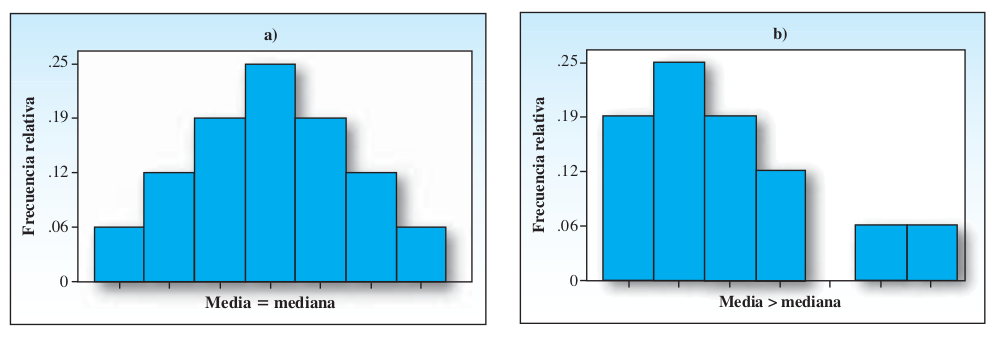
\includegraphics[width=\textwidth]{im7}
\end{center}

\end{frame}
%%%%%%%%%%%%%%%%%%%%%%%%%%%%%%%%%%%%%%%%%%%%%%%%%%%%%%%%%%%%%%%%%%%%%%%%%%%%%%%%%%%%%%%%%%%%%%%%%%%%%%%%%%%%%
\begin{frame}
\frametitle{Moda}
Otra forma de localizar el centro de una distribución es buscar el valor de x que se presenta con la frecuencia más alta. Esta medida del centro se denomina moda.

\begin{block}{Definición}
La moda es la categoría que se presenta con más frecuencia o el valor
de x que se presenta con más frecuencia. Cuando las mediciones en una variable continua se han agrupado como histograma de frecuencia o de frecuencia relativa, la clase con el pico más alto o frecuencia se llama clase modal, y el punto medio de esa clase se toma como la moda.
\end{block}
\end{frame}
%%%%%%%%%%%%%%%%%%%%%%%%%%%%%%%%%%%%%%%%%%%%%%%%%%%%%%%%%%%%%%%%%%%%%%%%%%%%%%%%%%%%%%%%%%%%%%%%%%%%%%%%%%%%%
\begin{frame}
\frametitle{Moda}
\begin{center}
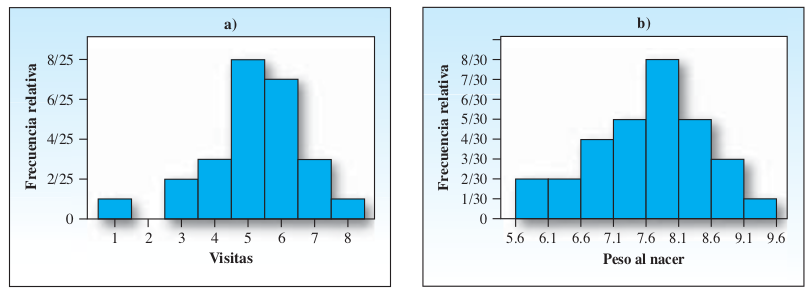
\includegraphics[width=\textwidth]{im8}
\end{center}
\end{frame}
%%%%%%%%%%%%%%%%%%%%%%%%%%%%%%%%%%%%%%%%%%%%%%%%%%%%%%%%%%%%%%%%%%%%%%%%%%%%%%%%%%%%%%%%%%%%%%%%%%%%%%%%%%%%%
\begin{frame}
\frametitle{Moda}
Es posible que una distribución de mediciones tenga más de una moda. Estas modas aparecerían como “picos locales” en la distribución de frecuencia relativa. Por ejemplo, si fuéramos a tabular la longitud de los peces sacados de un lago durante una temporada, podríamos obtener una distribución bimodal, posiblemente reflejando una mezcla de peces jóvenes y viejos en la población. A veces las distribuciones bimodales de tamaños o pesos reflejan una mezcla de mediciones tomadas en machos y hembras. En cualquier caso, un conjunto o distribución de mediciones puede tener más de una moda.
\end{frame}
%%%%%%%%%%%%%%%%%%%%%%%%%%%%%%%%%%%%%%%%%%%%%%%%%%%%%%%%%%%%%%%%%%%%%%%%%%%%%%%%%%%%%%%%%%%%%%%%%%%%%%%%%%%%%
\begin{frame}
\frametitle{Ejercicio}
Tiempo transcurrido entre la toma de pedido y el servicio a la mesa de los restaurantes fueron registrados 
\begin{center}
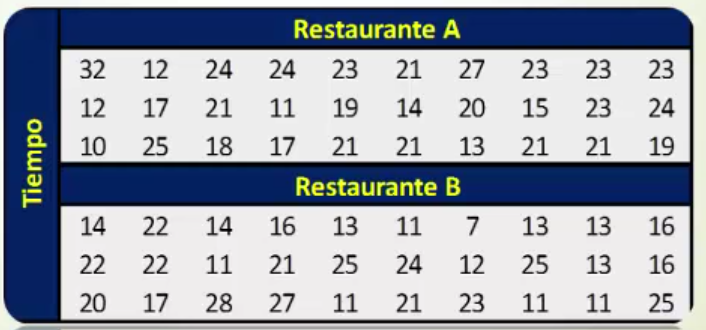
\includegraphics[scale=0.4]{im9}
\end{center}
¿Cuál restaurante considera usted que presta un mejor servicio y por qué?
\end{frame}
%%%%%%%%%%%%%%%%%%%%%%%%%%%%%%%%%%%%%%%%%%%%%%%%%%%%%%%%%%%%%%%%%%%%%%%%%%%%%%%%%%%%%%%%%%%%%%%%%%%%%%%%%%%%%
\begin{frame}
\frametitle{Ejercicio}
Resultados
\begin{center}
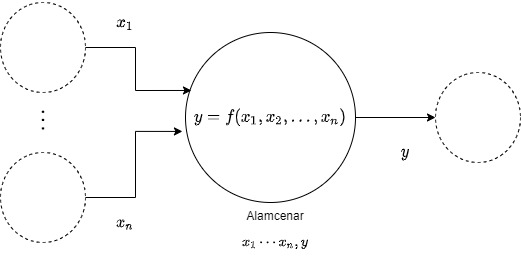
\includegraphics[scale=0.5]{im10}
\end{center}
\end{frame}
%%%%%%%%%%%%%%%%%%%%%%%%%%%%%%%%%%%%%%%%%%%%%%%%%%%%%%%%%%%%%%%%%%%%%%%%%%%%%%%%%%%%%%%%%%%%%%%%%%%%%%%%%%%%%
\begin{frame}
\frametitle{Medidas de variabilidad}
Los conjuntos de datos pueden tener el mismo centro pero con aspecto diferente por la forma en que los números se dispersan desde el centro. Considere las dos distribuciones que se muestran en la fi gura 2.6. Ambas distribuciones están centradas en $x=4$, pero hay una gran diferencia en la forma en que las mediciones se dispersan o varían.
\begin{center}
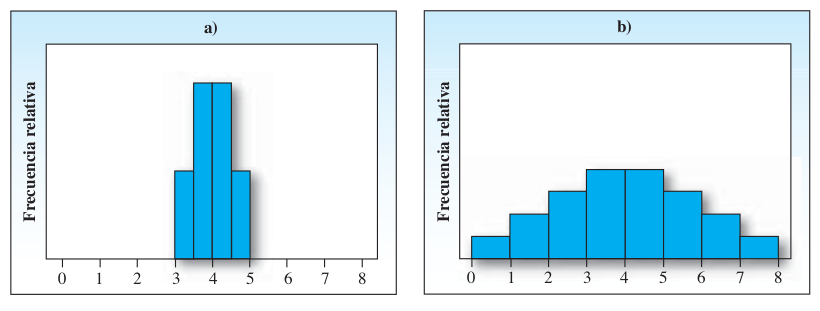
\includegraphics[width=\textwidth]{im11}
\end{center}
\end{frame}

%%%%%%%%%%%%%%%%%%%%%%%%%%%%%%%%%%%%%%%%%%%%%%%%%%%%%%%%%%%%%%%%%%%%%%%%%%%%%%%%%%%%%%%%%%%%%%%%%%%%%%%%%%%%%
\begin{frame}
\frametitle{Rango}
\begin{block}{Definición}
El rango, R, de un conjunto de n mediciones se define como la diferencia entre la medición más grande y la más pequeña.
\end{block}
\vspace{1em}

Para los datos de peso al nacer de la tabla, las mediciones varían de 5.6 a 9.4. Por tanto, el rango es $9.4-5.6 =3.8$.
\begin{center}
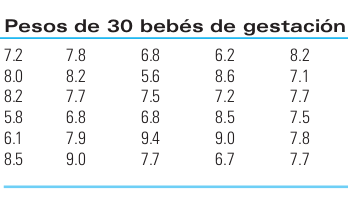
\includegraphics[scale=0.5]{im4}
\end{center}
\end{frame}

%%%%%%%%%%%%%%%%%%%%%%%%%%%%%%%%%%%%%%%%%%%%%%%%%%%%%%%%%%%%%%%%%%%%%%%%%%%%%%%%%%%%%%%%%%%%%%%%%%%%%%%%%%%%%
\begin{frame}
\frametitle{Rango}
El rango es fácil de calcular, fácil de interpretar
y es una medida adecuada de variación para conjuntos pequeños de datos. Pero, para conjuntos grandes, el rango no es una medida adecuada de variabilidad. Por ejemplo, las dos distribuciones de frecuencia relativa de la figura tienen el mismo rango pero muy diferentes formas y variabilidad.
\begin{center}
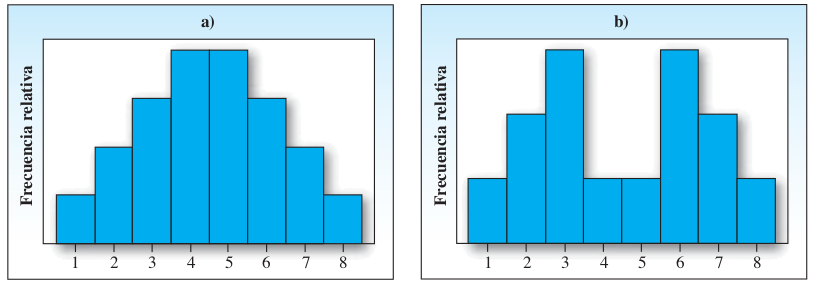
\includegraphics[width=\textwidth]{im12}
\end{center}
\end{frame}


%%%%%%%%%%%%%%%%%%%%%%%%%%%%%%%%%%%%%%%%%%%%%%%%%%%%%%%%%%%%%%%%%%%%%%%%%%%%%%%%%%%%%%%%%%%%%%%%%%%%%%%%%%%%%
\begin{frame}
\frametitle{Varianza}
¿Hay una medida de variabilidad que sea más sensible que el rango?
\begin{columns}
\column{0.6\textwidth}
\begin{center}
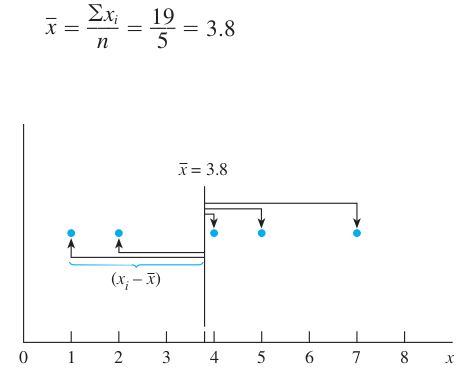
\includegraphics[width=\textwidth]{im13}
\end{center}

\column{0.4\textwidth}
\begin{center}
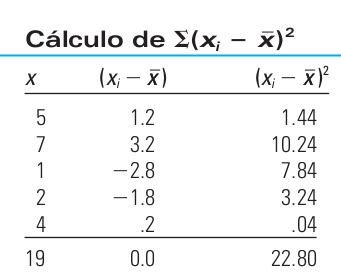
\includegraphics[width=\textwidth]{im14}
\end{center}
\end{columns}

\end{frame}
%%%%%%%%%%%%%%%%%%%%%%%%%%%%%%%%%%%%%%%%%%%%%%%%%%%%%%%%%%%%%%%%%%%%%%%%%%%%%%%%%%%%%%%%%%%%%%%%%%%%%%%%%%%%%
\begin{frame}
\frametitle{Varianza}
De la suma de desviaciones cuadradas, se calcula una sola medida llamada varianza. Para la varianza de una muestra usamos el símbolo $s^2$ y la varianza de una población $\sigma^2$. La varianza será relativamente grande para datos muy variables y relativamente pequeña para datos menos variables.
\begin{block}{Definición}
La \textbf{varianza de una población} de $N$ mediciones es el promedio de los
cuadrados de las desviaciones de las mediciones alrededor de su media $\mu$. La varianza poblacional se denota con $\sigma^2$ y está dada por la fórmula
\begin{equation*}
\sigma^2= \frac{\sum {(x_{i}- \mu)}^2}{N}
\end{equation*}
\end{block}

\end{frame}
%%%%%%%%%%%%%%%%%%%%%%%%%%%%%%%%%%%%%%%%%%%%%%%%%%%%%%%%%%%%%%%%%%%%%%%%%%%%%%%%%%%%%%%%%%%%%%%%%%%%%%%%%%%%%
\begin{frame}
\frametitle{Varianza}

\begin{block}{Definición}
La \textbf{varianza de una muestra} de $n$ mediciones es la suma de las desviaciones cuadradas de las mediciones alrededor la media $\bar{x}$ dividida entre $(n-1)$. La varianza muestral se denota con $s^2$ y está dada por la fórmula 

\begin{equation*}
s^2= \frac{\sum {(x_{i}- \bar{x})}^2}{n-1}
\end{equation*}
\end{block}

\end{frame}
%%%%%%%%%%%%%%%%%%%%%%%%%%%%%%%%%%%%%%%%%%%%%%%%%%%%%%%%%%%%%%%%%%%%%%%%%%%%%%%%%%%%%%%%%%%%%%%%%%%%%%%%%%%%%
\begin{frame}
\frametitle{Varianza}
Para el conjunto de $n = 5$ mediciones muestrales presentadas en la tabla
\begin{columns}
\column{0.6\textwidth}
suma
\begin{equation*}
\sum {(x_{i}- \bar{x})}^2=22.80
\end{equation*}
varianza muestral

\begin{equation*}
s^2= \frac{\sum {(x_{i}- \bar{x})}^2}{n-1}= \frac{22.80}{4}=5.70
\end{equation*}

\column{0.4\textwidth}
\begin{center}
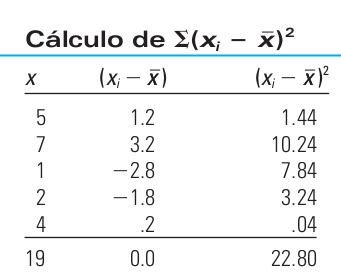
\includegraphics[width=\textwidth]{im14}
\end{center}
\end{columns}

\end{frame}
%%%%%%%%%%%%%%%%%%%%%%%%%%%%%%%%%%%%%%%%%%%%%%%%%%%%%%%%%%%%%%%%%%%%%%%%%%%%%%%%%%%%%%%%%%%%%%%%%%%%%%%%%%%%%
\begin{frame}
\frametitle{Desviación estándar}
La varianza se mide en términos del cuadrado de las unidades originales de medición. Tomando la raíz cuadrada de la varianza, obtenemos la desviación estándar, que regresa la medida de variabilidad a las unidades originales de medición.

\begin{block}{Definición}
La \textbf{desviación estándar} de un conjunto de mediciones es igual a la raíz
cuadrada positiva de la varianza.
\end{block}
\end{frame}
%%%%%%%%%%%%%%%%%%%%%%%%%%%%%%%%%%%%%%%%%%%%%%%%%%%%%%%%%%%%%%%%%%%%%%%%%%%%%%%%%%%%%%%%%%%%%%%%%%%%%%%%%%%%%
\begin{frame}
\frametitle{Notación}

\begin{center}
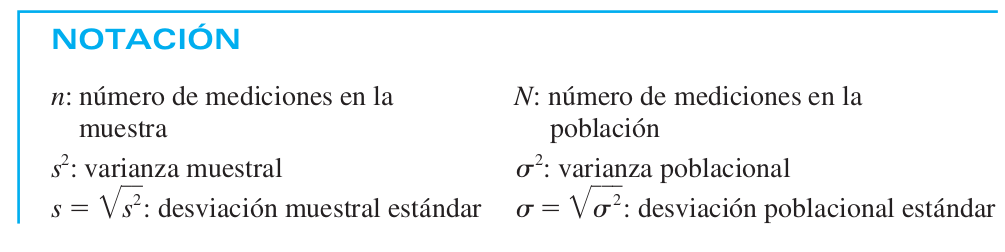
\includegraphics[width=\textwidth]{im15}
\end{center}

\end{frame}
%%%%%%%%%%%%%%%%%%%%%%%%%%%%%%%%%%%%%%%%%%%%%%%%%%%%%%%%%%%%%%%%%%%%%%%%%%%%%%%%%%%%%%%%%%%%%%%%%%%%%%%%%%%%%
\begin{frame}
\frametitle{Resumen}

\begin{center}
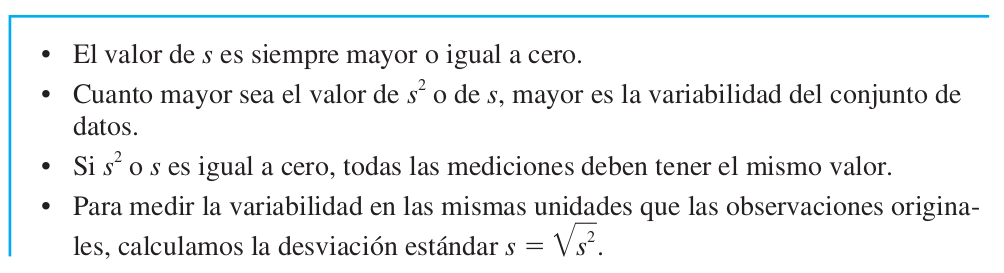
\includegraphics[width=\textwidth]{im16}
\end{center}

\end{frame}
%%%%%%%%%%%%%%%%%%%%%%%%%%%%%%%%%%%%%%%%%%%%%%%%%%%%%%%%%%%%%%%%%%%%%%%%%%%%%%%%%%%%%%%%%%%%%%%%%%%%%%%%%%%%%
\begin{frame}
\frametitle{Coeficiente de variación}
El coeficiente de variación es la relación entre la desviación típica de una muestra y su media.
\begin{equation*}
CV=\left( \frac{\sigma}{\bar{x}} \right) 100
\end{equation*}
El coeficiente de variación permite comparar las dispersiones de dos distribuciones distintas, siempre que sus medias sean positivas.

Mayor dispersión el valor del coeficiente de variación será mayor.
\end{frame}
%%%%%%%%%%%%%%%%%%%%%%%%%%%%%%%%%%%%%%%%%%%%%%%%%%%%%%%%%%%%%%%%%%%%%%%%%%%%%%%%%%%%%%%%%%%%%%%%%%%%%%%%%%%%%
\begin{frame}
\frametitle{Coeficiente de variación}
Una distribución tiene $\bar{x}=140$ y $\sigma =28.28$ y otra $\bar{x}=150$ y $\sigma =24$. ¿Cuál de las dos presenta mayor dispersión?

\begin{equation*}
\textup{CV}_{1}=\cfrac{28,28}{140}\cdot 100=20,2 \%
\end{equation*}
 
\begin{equation*}
\textup{CV}_{2}=\cfrac{24}{150}\cdot 100=16 \%
\end{equation*}
 
La primera distribución presenta mayor dispersión.

\end{frame}
%%%%%%%%%%%%%%%%%%%%%%%%%%%%%%%%%%%%%%%%%%%%%%%%%%%%%%%%%%%%%%%%%%%%%%%%%%%%%%%%%%%%%%%%%%%%%%%%%%%%%%%%%%%%%
\begin{frame}
\frametitle{Sobre la significancia práctica de la desviación estándar}

\begin{block}{Teorema de Chebyshev}
Dado un número $k$ mayor o igual a $1$ y un conjunto de n mediciones, al menos $[1 - (1/k^2)]$ de las mediciones estarán dentro de $k$ desviaciones estándar de su media.
\end{block}

Se construye un intervalo al medir una distancia $k\sigma$ a cualquier lado de la media $m$. El número $k$ puede ser cualquier número mientras sea mayor o igual a 1. Entonces el teorema de Chebyshev expresa que al menos $[1 - (1/k^2)]$ del número total $n$ de mediciones está en el intervalo construido.

\end{frame}
%%%%%%%%%%%%%%%%%%%%%%%%%%%%%%%%%%%%%%%%%%%%%%%%%%%%%%%%%%%%%%%%%%%%%%%%%%%%%%%%%%%%%%%%%%%%%%%%%%%%%%%%%%%%%
\begin{frame}
\frametitle{Teorema de Chebyshev}
Ilustración del teorema de Chebyshev
\begin{center}
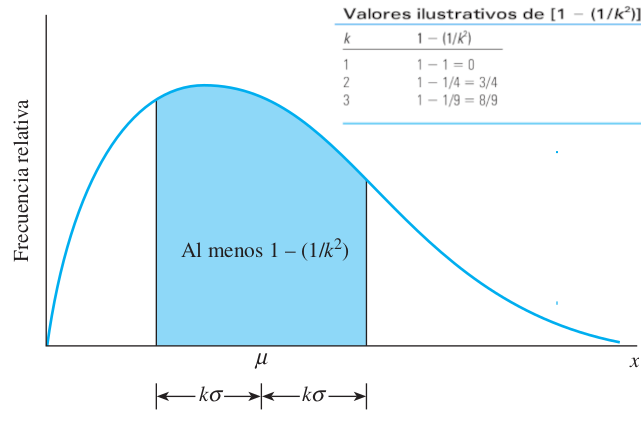
\includegraphics[width=0.8\textwidth]{im17}
\end{center}


\end{frame}
%%%%%%%%%%%%%%%%%%%%%%%%%%%%%%%%%%%%%%%%%%%%%%%%%%%%%%%%%%%%%%%%%%%%%%%%%%%%%%%%%%%%%%%%%%%%%%%%%%%%%%%%%%%%%
\begin{frame}
\frametitle{Teorema de Chebyshev}
Ilustración del teorema de Chebyshev
\begin{center}
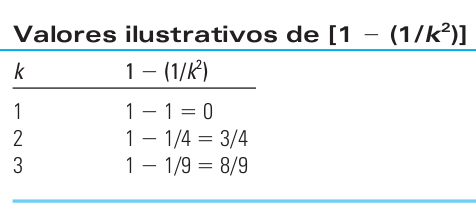
\includegraphics[scale=0.4]{im18}
\end{center}
\begin{center}
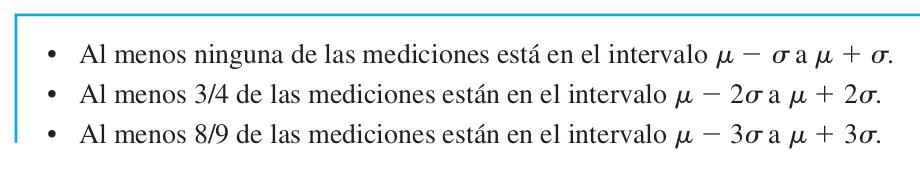
\includegraphics[width=\textwidth]{im19}
\end{center}

\end{frame}
%%%%%%%%%%%%%%%%%%%%%%%%%%%%%%%%%%%%%%%%%%%%%%%%%%%%%%%%%%%%%%%%%%%%%%%%%%%%%%%%%%%%%%%%%%%%%%%%%%%%%%%%%%%%%
\begin{frame}
\frametitle{Teorema de Chebyshev}
Ejemplo. La media y varianza de una muestra de $n = 25$ mediciones son $75$ y $100$, respectivamente. Use el teorema de Chebyshev para describir la distribución de mediciones.

Solución Nos dan $\bar{x} =75$ y $s^2 = 100$. La desviación estándar es $s =\sqrt{100}=10$. La distribución de mediciones está centrada alrededor de x = 75, y el teorema de Chebyshev establece que:
\begin{itemize}
\item Al menos $3/4$ de las 25 mediciones están en el intervalo $\bar{x} \pm  2s = 75 \pm 2(10)$, esto es, $55$ a $95$.

\item Al menos $8/9$ de las mediciones están en el intervalo $\bar{x} \pm  3s = 75 \pm 3(10)$, esto es, 45 a 105.
\end{itemize}


\end{frame}
%%%%%%%%%%%%%%%%%%%%%%%%%%%%%%%%%%%%%%%%%%%%%%%%%%%%%%%%%%%%%%%%%%%%%%%%%%%%%%%%%%%%%%%%%%%%%%%%%%%%%%%%%%%%%
\begin{frame}
\frametitle{Regla empírica}
Como el teorema de Chebyshev se aplica a cualquier distribución, es muy conservador. Ésta es la razón por la que hacemos hincapié en “al menos $1 - (1/k ^2)$” en este teorema. Otra regla para describir la variabilidad de un conjunto de datos no funciona para todos los conjuntos de datos, pero funciona muy bien para datos que “se apilan” en la conocida forma de montículo de la figura

\begin{center}
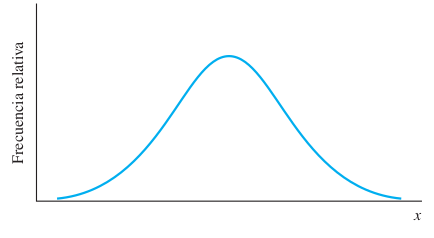
\includegraphics[scale=0.4]{im20}
\end{center}
\end{frame}
%%%%%%%%%%%%%%%%%%%%%%%%%%%%%%%%%%%%%%%%%%%%%%%%%%%%%%%%%%%%%%%%%%%%%%%%%%%%%%%%%%%%%%%%%%%%%%%%%%%%%%%%%%%%%
\begin{frame}
\frametitle{Regla empírica}
\begin{center}
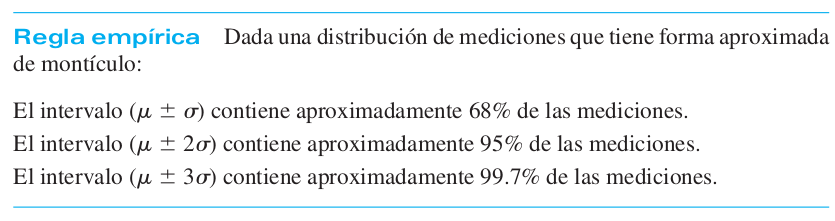
\includegraphics[scale=0.4]{im21}
\end{center}


\end{frame}
%%%%%%%%%%%%%%%%%%%%%%%%%%%%%%%%%%%%%%%%%%%%%%%%%%%%%%%%%%%%%%%%%%%%%%%%%%%%%%%%%%%%%%%%%%%%%%%%%%%%%%%%%%%%%
\begin{frame}
\frametitle{Regla empírica}
Ejercicio 

En un estudio de tiempo efectuado en una planta manufacturera, el tiempo para completar una operación especificada se mide para cada uno de los $n= 40$ trabajadores. Se encuentra que la media y la desviación estándar son 12.8 y 1.7, respectivamente. Describa los datos muestrales usando la Regla empírica.


\end{frame}
%%%%%%%%%%%%%%%%%%%%%%%%%%%%%%%%%%%%%%%%%%%%%%%%%%%%%%%%%%%%%%%%%%%%%%%%%%%%%%%%%%%%%%%%%%%%%%%%%%%%%%%%%%%%%
\begin{frame}
\frametitle{Regla empírica}
\begin{center}
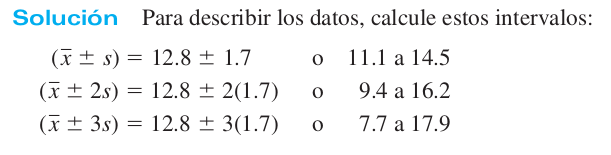
\includegraphics[scale=0.4]{im22}
\end{center}
De acuerdo con la Regla empírica, se espera que aproximadamente 68\% de las mediciones caigan en el intervalo de 11.1 a 14.5, aproximadamente 95\% caigan en el intervalo de 9.4 a 16.2, y aproximadamente 99.7\% caigan en el intervalo de 7.7 a 17.9.

\end{frame}
%%%%%%%%%%%%%%%%%%%%%%%%%%%%%%%%%%%%%%%%%%%%%%%%%%%%%%%%%%%%%%%%%%%%%%%%%%%%%%%%%%%%%%%%%%%%%%%%%%%%%%%%%%%%%
\begin{frame}
\frametitle{Ejercicio}
Los maestros-estudiantes son capacitados para desarrollar planes de lecciones, en la suposición de que el plan escrito les ayudará a trabajar de manera satisfactoria en el salón de clases. En un estudio para evaluar la relación entre planes de lección escritos y su implementación en el salón de clases, se calificaron 25 planes de lección en una escala de 0 a 34 de acuerdo a una Lista de verificación de Plan de lección. Las 25 calificaciones se
muestran en la tabla. Use el teorema de Chebyshev y la Regla empírica (si es aplicable) para describir la distribución de estas calificaciones de evaluación.
\begin{center}
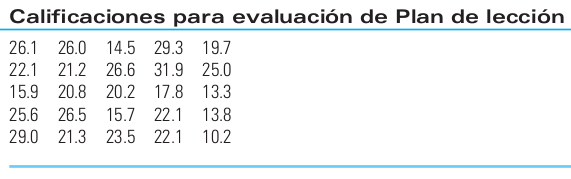
\includegraphics[scale=0.4]{im23}
\end{center}


\end{frame}
%%%%%%%%%%%%%%%%%%%%%%%%%%%%%%%%%%%%%%%%%%%%%%%%%%%%%%%%%%%%%%%%%%%%%%%%%%%%%%%%%%%%%%%%%%%%%%%%%%%%%%%%%%%%%
\begin{frame}
\frametitle{Mediciones de posición relativa }
A veces es necesario conocer la posición de una observación respecto a otras de un conjunto de datos.

\begin{block}{Definición}
El \textbf{puntaje z muestral} es una medida de posición relativa definida
por
\begin{equation*}
\text{puntaje } z = \frac{x-\bar{x}}{s}
\end{equation*}
\end{block}

Un puntaje z mide la distancia entre una observación y la media, medidas en unidades de desviación estándar.

\end{frame}
%%%%%%%%%%%%%%%%%%%%%%%%%%%%%%%%%%%%%%%%%%%%%%%%%%%%%%%%%%%%%%%%%%%%%%%%%%%%%%%%%%%%%%%%%%%%%%%%%%%%%%%%%%%%%
\begin{frame}
\frametitle{Mediciones de posición relativa }
Por ejemplo, suponga que la media y desviación estándar de los puntajes de examen (basados en un total de 35 puntos) son 25 y 4, respectivamente. El puntaje z para una calificación de 30 se calcula como sigue:

\begin{equation*}
\text{puntaje } z = \frac{x-\bar{x}}{s}=\frac{30-25}{4}=1.25
\end{equation*}

El puntaje de 30 está a 1.25 desviaciones estándar arriba de la media $(30 = \bar{x}+1.25s)$.
\end{frame}
%%%%%%%%%%%%%%%%%%%%%%%%%%%%%%%%%%%%%%%%%%%%%%%%%%%%%%%%%%%%%%%%%%%%%%%%%%%%%%%%%%%%%%%%%%%%%%%%%%%%%%%%%%%%%
\begin{frame}
\frametitle{Mediciones de posición relativa }
\begin{center}
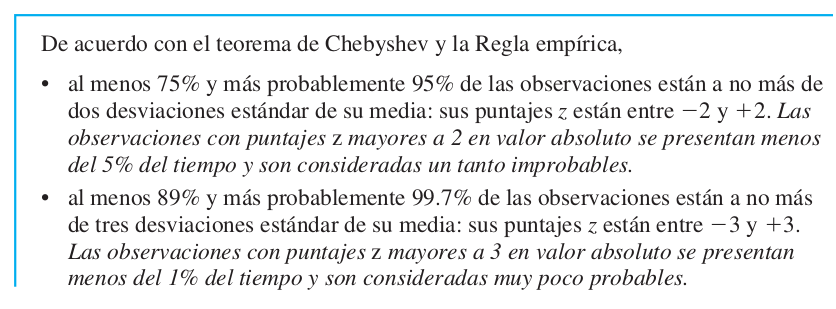
\includegraphics[scale=0.4]{im24}
\end{center}
\end{frame}
%%%%%%%%%%%%%%%%%%%%%%%%%%%%%%%%%%%%%%%%%%%%%%%%%%%%%%%%%%%%%%%%%%%%%%%%%%%%%%%%%%%%%%%%%%%%%%%%%%%%%%%%%%%%%
\begin{frame}
\frametitle{Percentil}
Un percentil es otra medida de posición relativa y se usa con más frecuencia para conjuntos grandes de datos. (Los percentiles no son muy útiles para conjuntos pequeños de datos).

\begin{block}{Definición}
Un conjunto de n mediciones de la variable $x$ se ha reacomodado en
orden de magnitud. El p-ésimo percentil es el valor de $x$ que es mayor a $p\%$ de las mediciones y es menor que el restante $(100 - p)\%$.
\end{block}


\end{frame}
%%%%%%%%%%%%%%%%%%%%%%%%%%%%%%%%%%%%%%%%%%%%%%%%%%%%%%%%%%%%%%%%%%%%%%%%%%%%%%%%%%%%%%%%%%%%%%%%%%%%%%%%%%%%%
\begin{frame}
\frametitle{Percentil}
Supongamos que usted ha sido notificado que su calificación de 610, en el Examen verbal de graduación, lo ha colocado en el 60avo percentil en la distribución de calificaciones. ¿Dónde está su calificación de 610 en relación a las calificaciones de los otros que tomaron el examen?

\vspace{1em}
Solución Calificar en el 60avo percentil significa que $60\%$ de todas las calificaciones de examen fueron más bajas que la calificación de usted y $40\%$ fueron más altas.

\end{frame}
%%%%%%%%%%%%%%%%%%%%%%%%%%%%%%%%%%%%%%%%%%%%%%%%%%%%%%%%%%%%%%%%%%%%%%%%%%%%%%%%%%%%%%%%%%%%%%%%%%%%%%%%%%%%%
\begin{frame}
\frametitle{Percentil}
En general, el 60avo percentil para la variable x es un punto en el eje horizontal de la distribución de datos que es mayor a 60\% de las mediciones y menor que las otras.

\begin{center}
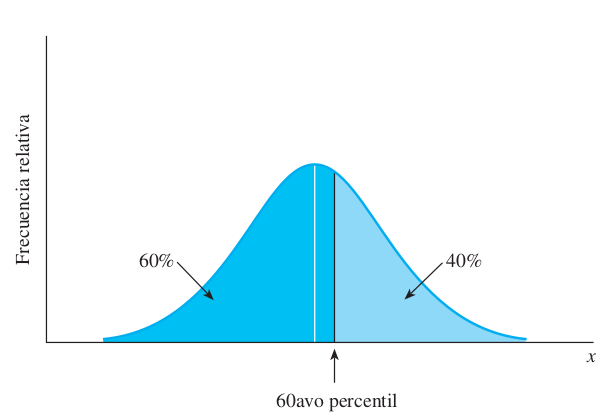
\includegraphics[scale=0.4]{im25}
\end{center}

\end{frame}
%%%%%%%%%%%%%%%%%%%%%%%%%%%%%%%%%%%%%%%%%%%%%%%%%%%%%%%%%%%%%%%%%%%%%%%%%%%%%%%%%%%%%%%%%%%%%%%%%%%%%%%%%%%%%
\begin{frame}
\frametitle{Percentil-Cuartil}

\begin{itemize}
\item La mediana es igual que el 50avo percentil.
\item Los percentiles 25avo y 75avo, llamados cuartiles inferior y superior
\item Veinticinco por ciento de las mediciones serán menores que el cuartil inferior (primero).
\item 50\% serán menores que la mediana (el segundo cuartil).
\item 75\% serán menores que el cuartil superior (tercero).
\end{itemize}

\end{frame}
%%%%%%%%%%%%%%%%%%%%%%%%%%%%%%%%%%%%%%%%%%%%%%%%%%%%%%%%%%%%%%%%%%%%%%%%%%%%%%%%%%%%%%%%%%%%%%%%%%%%%%%%%%%%%
\begin{frame}
\frametitle{Cuartil}

\begin{center}
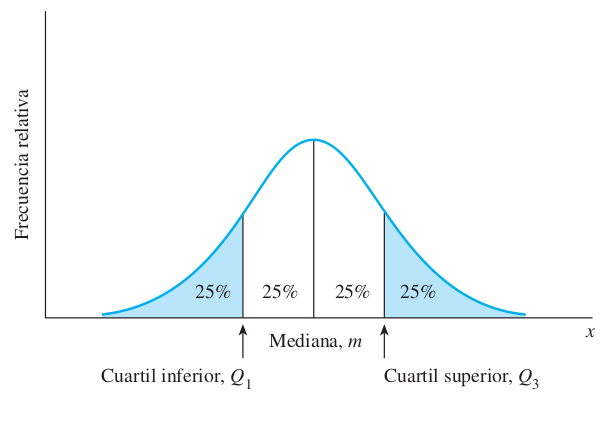
\includegraphics[scale=0.4]{im26}
\end{center}

\end{frame}
%%%%%%%%%%%%%%%%%%%%%%%%%%%%%%%%%%%%%%%%%%%%%%%%%%%%%%%%%%%%%%%%%%%%%%%%%%%%%%%%%%%%%%%%%%%%%%%%%%%%%%%%%%%%%
\begin{frame}
\frametitle{Cuartil}

\begin{block}{Definición}
Un conjunto de $n$ mediciones en la variable $x$ se ha acomodado en orden
de magnitud. El \textbf{cuartil inferior (primer cuartil), $Q_{1}$ }, es el valor de $x$ que es mayor a un cuarto de las mediciones y es menor que los restantes tres cuartos. El s\textbf{egundo cuartil} es la mediana. El \textbf{cuartil superior (tercer cuartil), $Q_{3}$ }, es el valor de $x$ que es mayor a tres cuartos de las mediciones y es menor que el restante un cuarto.
\end{block}

\end{frame}
%%%%%%%%%%%%%%%%%%%%%%%%%%%%%%%%%%%%%%%%%%%%%%%%%%%%%%%%%%%%%%%%%%%%%%%%%%%%%%%%%%%%%%%%%%%%%%%%%%%%%%%%%%%%%
\begin{frame}
\frametitle{Cuartil}

\begin{center}
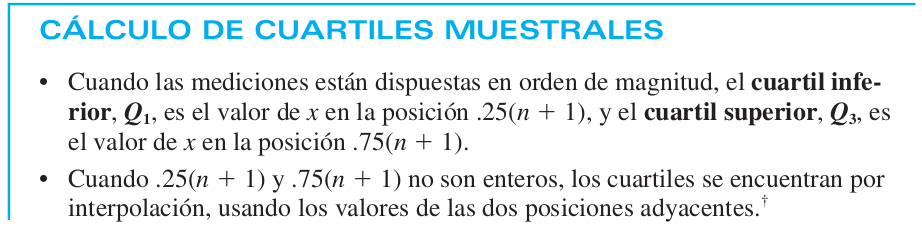
\includegraphics[width=\textwidth]{im27}
\end{center}


\end{frame}
%%%%%%%%%%%%%%%%%%%%%%%%%%%%%%%%%%%%%%%%%%%%%%%%%%%%%%%%%%%%%%%%%%%%%%%%%%%%%%%%%%%%%%%%%%%%%%%%%%%%%%%%%%%%%
\begin{frame}
\frametitle{Cuartil}

\begin{center}
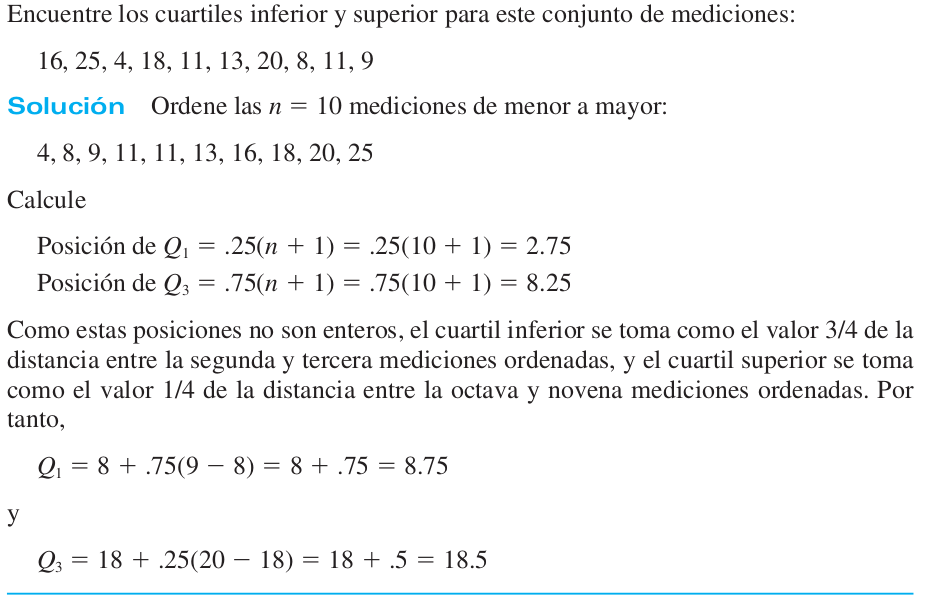
\includegraphics[width=\textwidth]{im28}
\end{center}


\end{frame}
%%%%%%%%%%%%%%%%%%%%%%%%%%%%%%%%%%%%%%%%%%%%%%%%%%%%%%%%%%%%%%%%%%%%%%%%%%%%%%%%%%%%%%%%%%%%%%%%%%%%%%%%%%%%%
\begin{frame}
\frametitle{Intercuartil}
Como la mediana y los cuartiles dividen la distribución de datos en cuatro partes, cada una de ellas conteniendo alrededor de 25\% de las mediciones, $Q_1$ y $Q_3$ son las fronteras superior e inferior para el 50\% central de la distribución. Podemos medir el rango de este “50\% central” de la distribución usando una medida numérica llamada rango intercuartil.

\begin{block}{Definición}
El rango intercuartil (IQR) para un conjunto de mediciones es la diferencia entre los cuartiles superior e inferior; esto es, $IQR = Q_3 - Q_1$ .
\end{block}
\end{frame}
%%%%%%%%%%%%%%%%%%%%%%%%%%%%%%%%%%%%%%%%%%%%%%%%%%%%%%%%%%%%%%%%%%%%%%%%%%%%%%%%%%%%%%%%%%%%%%%%%%%%%%%%%%%%%
\begin{frame}
\frametitle{El resumen de cinco números y la gráfica de caja}


\begin{center}
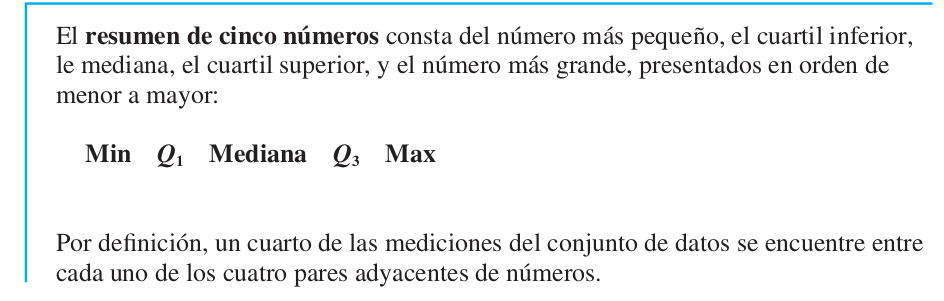
\includegraphics[width=\textwidth]{im29}
\end{center}

\end{frame}
%%%%%%%%%%%%%%%%%%%%%%%%%%%%%%%%%%%%%%%%%%%%%%%%%%%%%%%%%%%%%%%%%%%%%%%%%%%%%%%%%%%%%%%%%%%%%%%%%%%%%%%%%%%%%
\begin{frame}
\frametitle{El resumen de cinco números y la gráfica de caja}


\begin{center}
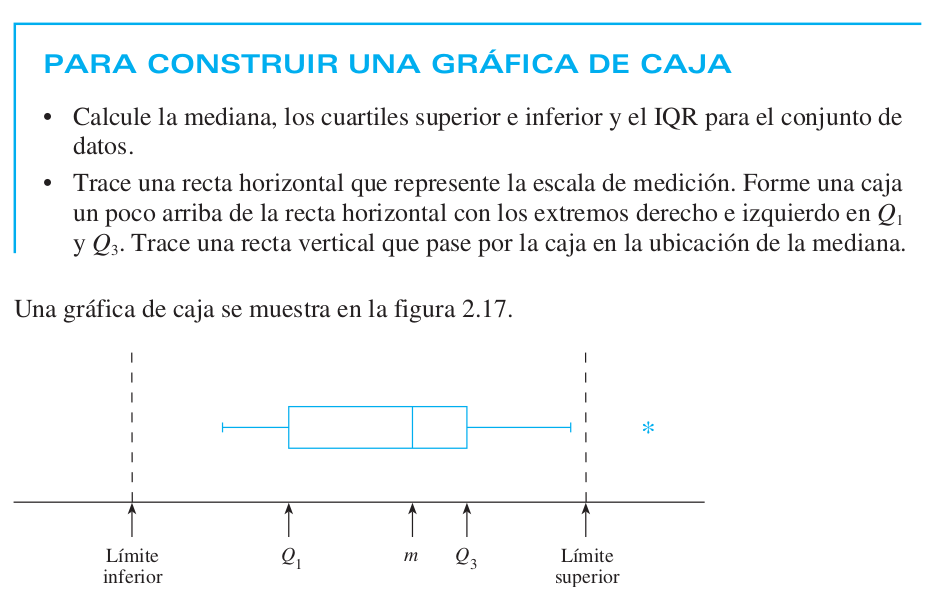
\includegraphics[width=\textwidth]{im30
}
\end{center}

\end{frame}
%%%%%%%%%%%%%%%%%%%%%%%%%%%%%%%%%%%%%%%%%%%%%%%%%%%%%%%%%%%%%%%%%%%%%%%%%%%%%%%%%%%%%%%%%%%%%%%%%%%%%%%%%%%%%
\end {document}



                                                  






